\documentclass[12pt,a4paper]{article}
\usepackage[utf8]{inputenc} %polskie znaki
\usepackage[T1]{fontenc}	%polskie znaki
\usepackage{amsmath}		%matematyczne znaczki :3
\usepackage{enumerate}		%Dodatkowe opcje do funkcji enumerate
\usepackage{geometry} 		%Ustawianie marginesow
\usepackage{graphicx}		%Grafika
\usepackage{wrapfig}		%Grafika obok textu
\usepackage{float}			%Allows H in fugire
\pagestyle{empty} 			%usuwa nr strony

\newgeometry{tmargin=2cm, bmargin=2cm, lmargin=2cm, rmargin=2cm} 

\begin{document}
	\begin{center}
		\LARGE Rachunek prawdopodobieństwa - karta pracy
	\end{center}
	\vspace{1.5cm}
	\begin{flushright}
		\textbf{2 TERMIN}
	\end{flushright}
	\begin{tabular}{p{13cm} r}
		Imię i nazwisko: ............................................................................
		&[....../30pkt]\\ 
		\vspace{0.5cm}
	\end{tabular}
	\begin{enumerate}[1.]
		\item  \begin{tabular}{p{13cm} r}
			Oblicz ile jest 6-cyfrowych kodów pin, w którym ostatnia cyfra jest parzysta, druga jest taka sama jak trzecia, pierwsza, czwarta i piąta są różne między sobą. &[2pkt]\\ 
		\end{tabular}
		
		\item  \begin{tabular}{p{13cm} r}
			W pewnej urnie jest 7 kul białych, 3 czarne i 5 niebieskich - wszystkie są ponumerowane. Losujemy z tej urny jednocześnie 3 kule. Na ile sposobów można wylosować kule tak, aby:  &[4pkt]\\ 
		\end{tabular}
		
		\begin{enumerate}[a)]
			\item w sumie to nie ma warunku (moga jakkolwiek zostać wybrane)
			\item wylosowane kule będą tego samego koloru
			\item nie będzie żadnej kuli białej
			\item wszystkie kule bedę różnego koloru
		\end{enumerate}
		
		\item  \begin{tabular}{p{13cm} r}
			Do przedziału (zobacz rysunek) wchodzi 8 osób (w tym Agata i Bartek). Oblicz na ile sposobów mogę wsiąść te osoby: &[4pkt]\\ 
		\end{tabular}
	
	\begin{enumerate}[a)]
		\item dowolnie
		\item tak aby Agata i Bartek siedzieli obok siebie (obok nie na przeciwko)
		\item tak aby Agata i Bartek byli zwróceni w strone kierunku jazdy
		\item tak aby Agata siedziała przy oknie, a Bartek tyłem do kierunku jazdy
	\end{enumerate}

\begin{figure}[h]
	\centering
	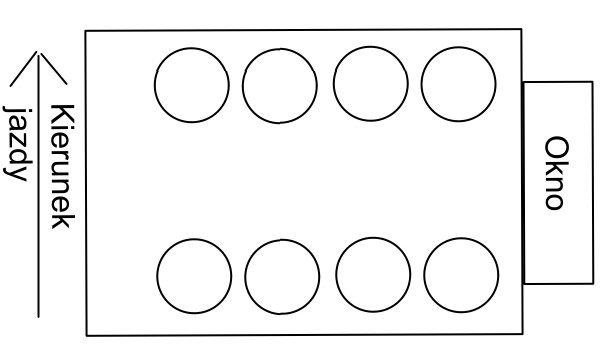
\includegraphics[scale=0.6]{prt1.jpeg}
\end{figure}

\newpage
	
		\item  \begin{tabular}{p{13cm} r}
		W schronisku jest 20 psów gotowych do adopcji, wśród nich Romek. Pewnego dnia do schroniska przyszło 6 par zdecydowanych na adopcje dokładnie jednego psa. Oblicz prawdopodobieństwo, że Romek będzie tego dnia miał nowy dom.  &[2pkt]\\ 
	\end{tabular}

		\item  \begin{tabular}{p{13cm} r}
	Oblicz prawdopodobieństwo, że przy dwukrotnych rzucie sześcienną kostką do gry suma oczek będzie więszka niż 8.  &[2pkt]\\ 
		\end{tabular}
	
	\item  \begin{tabular}{p{13cm} r}
		Oblicz ile wyrazów (mających sens lub nie) można utworzyć z wyrazu \textbf{KUKUŁKA}.  &[3pkt]\\ 
	\end{tabular}
	
		\item  \begin{tabular}{p{13cm} r}
		Oblicz medianę, dominantę i średnią arytmetyczną wieku studentów z tabeli &[3pkt]\\ 
	\end{tabular}

	\begin{tabular}{|c|c|c|c|c|c|c|}
		\hline
		Wiek&19&20&21&23&25&32\\
		\hline
		Liczba studentów&4&12&6&5&3&2\\
		\hline
	\end{tabular}

	\end{enumerate}
	
\end{document}
